This section reports on the results of the TRITIUM-IFIC 2 prototype during its installation in the IFIC laboratory.  The signal and background energy spectra are shown in Figure \ref{subfig:SignalBackgroundEnergySpectraTritiumIFIC2}. As it was mentioned in section \ref{subsec:TritiumIFIC2}, the signal prototype was filled with a tritiated water solution with an activity of $10~\kilo\becquerel/\liter$ and the background prototype was filled with ultrapure water. The difference between both spectra corresponds to the energy spectrum of tritium, Figure \ref{subfig:TritiumEnergySpectraTritiumIFIC2}. The rates obtained from these three spectra are given in Table \ref{tab:CountsPerSecondTRITIUMIFIC2}. 

\begin{figure}
\centering
    \begin{subfigure}[b]{0.73\textwidth}
    \centering
    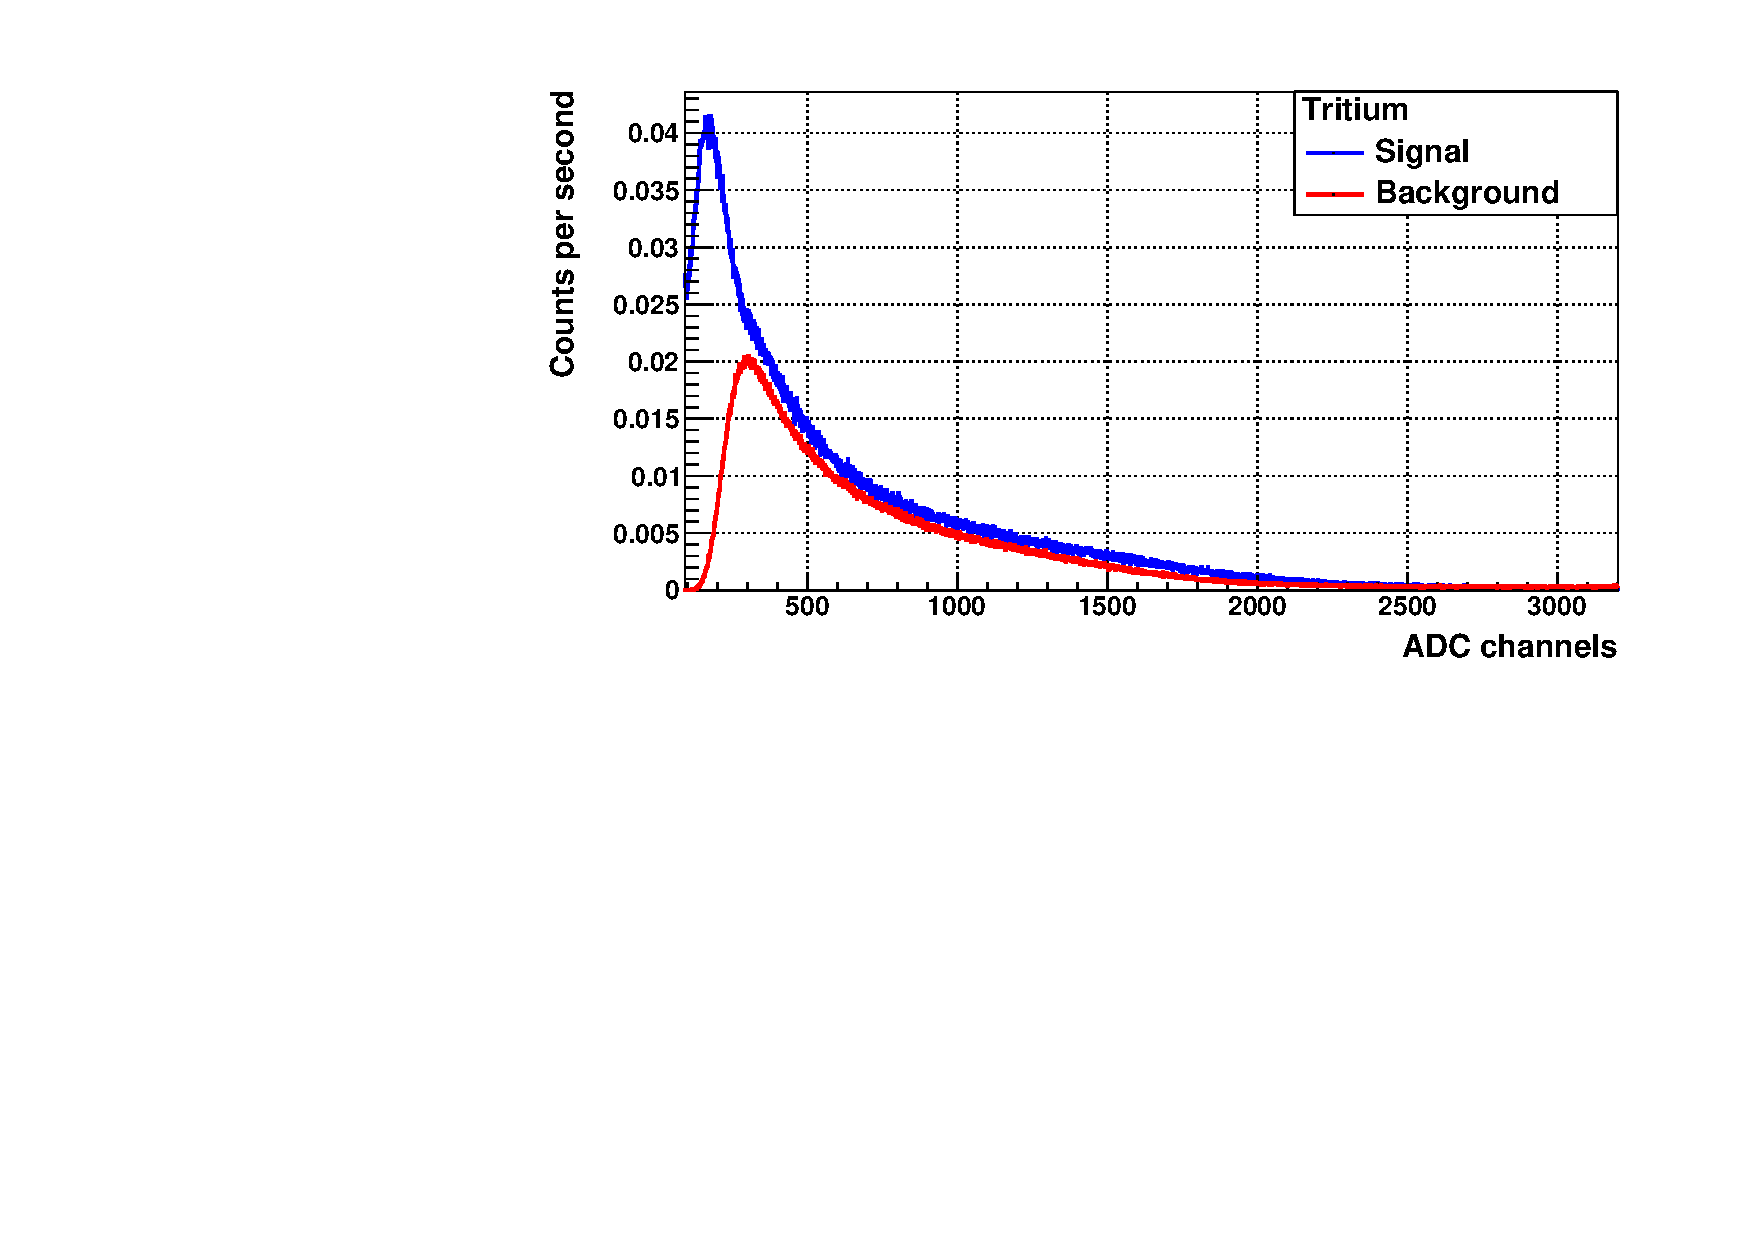
\includegraphics[width=\textwidth]{7ExperimentalResultsDetectors/71ExperimentalResultsLaboratory/714TRITIUMIFIC2/TritiumIFIC2SignalsHigherZOOM_NP.pdf}  
    \caption{\label{subfig:SignalBackgroundEnergySpectraTritiumIFIC2}}
    \end{subfigure}
    \hfill
    \begin{subfigure}[b]{0.73\textwidth}
    \centering
    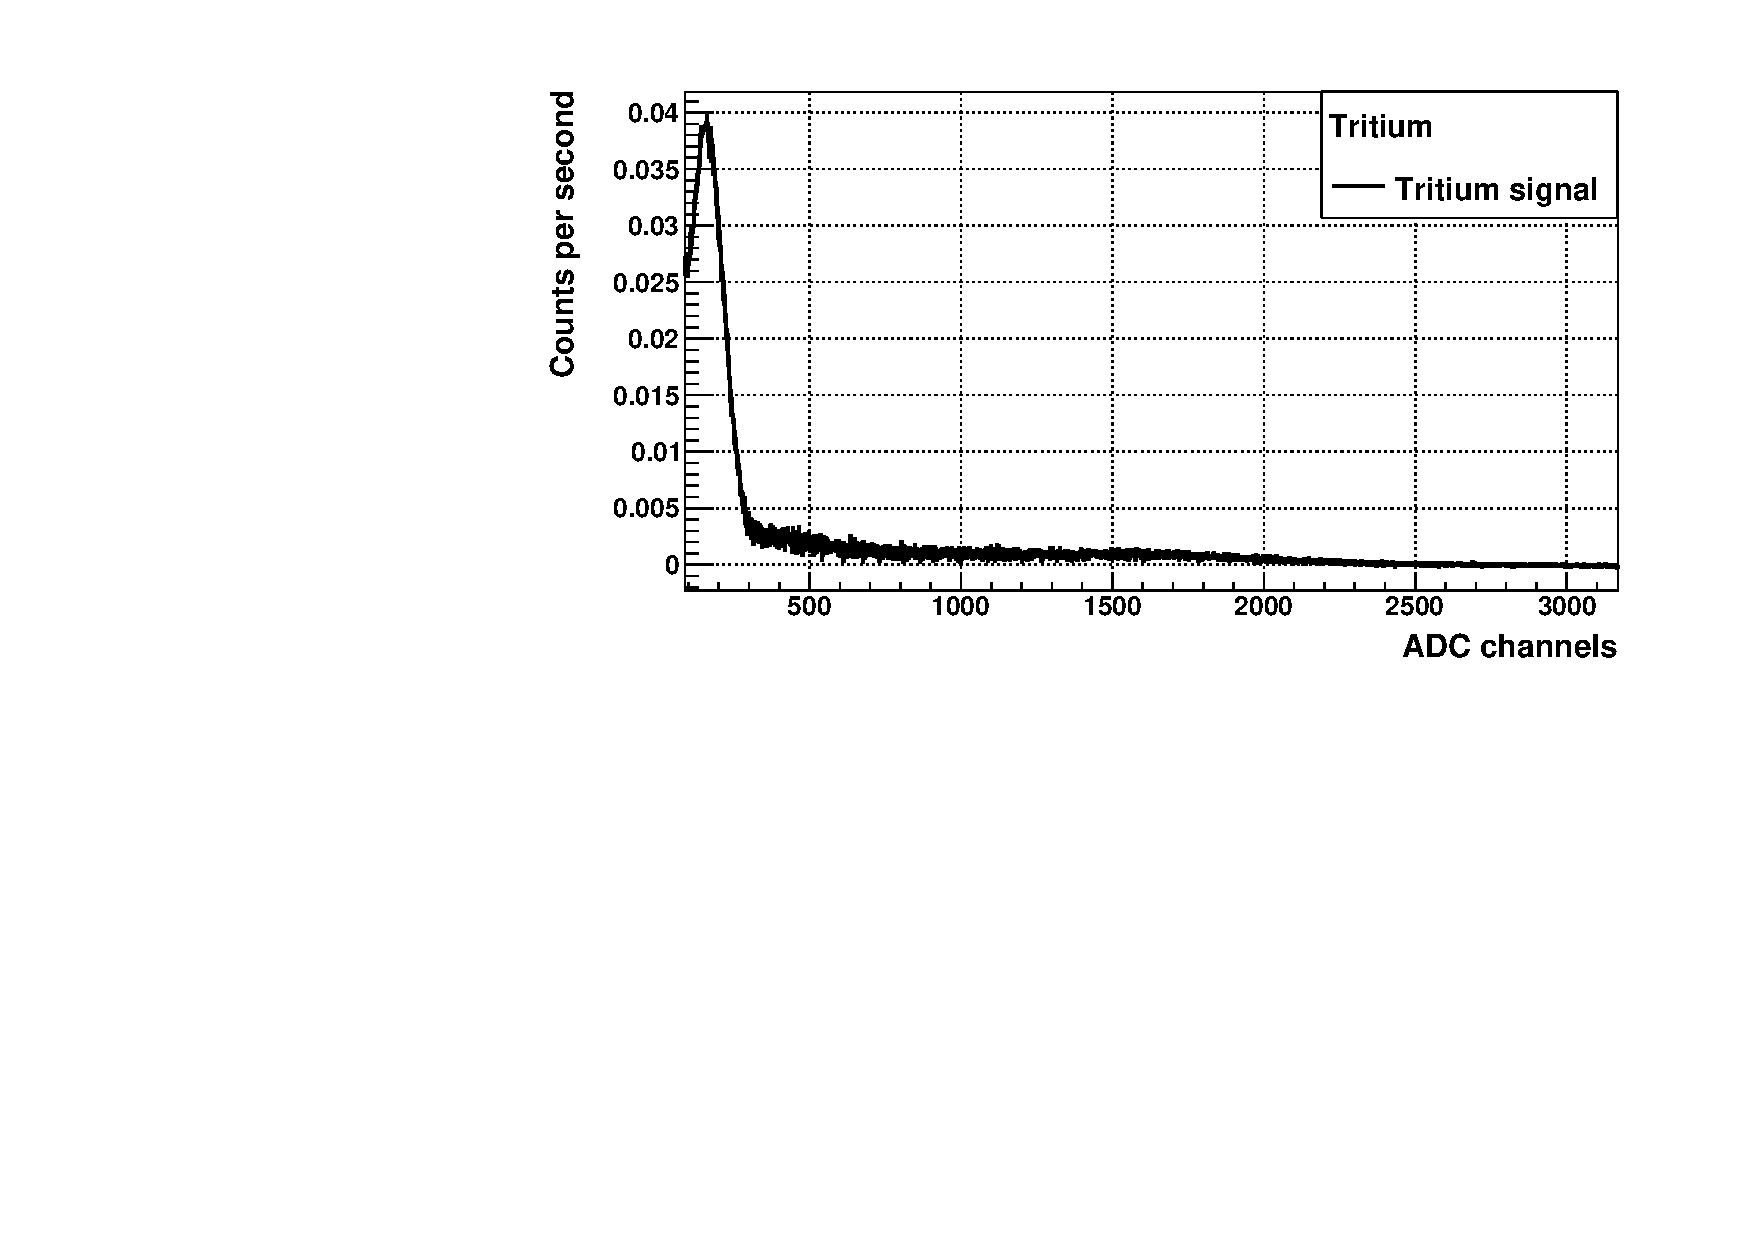
\includegraphics[width=\textwidth]{7ExperimentalResultsDetectors/71ExperimentalResultsLaboratory/714TRITIUMIFIC2/TritiumIFIC2ClearHigherZOOM_NP.pdf}  
    \caption{\label{subfig:TritiumEnergySpectraTritiumIFIC2}}
    \end{subfigure}
 \caption{Energy spectra measured with TRITIUM-IFIC 2 prototype. a) Signal and background energy spectra. b) Tritium energy spectrum.}
 \label{fig:EnergySpectraTRITIUMIFIC2}
\end{figure}

\begin{table}[htbp]
\centering{}%
\begin{tabular}{cc}
\toprule 
Spectrum & Counts/second \tabularnewline
\midrule
\midrule 
Signal prototype & $19.05 \pm 0.18$ \tabularnewline
Background prototype & $11.54 \pm 0.14$ \tabularnewline  
Tritium counts & $7.11 \pm 0.23$ \tabularnewline
\bottomrule
\end{tabular}
\caption{Counting rates measured by TRITIUM-IFIC 2 prototype.}
\label{tab:CountsPerSecondTRITIUMIFIC2}
\end{table}
The tritium detection efficiency obtained for this prototype is $(7.11 \pm 0.28)\cdot{} 10^{-1}~\liter\second^{-1}\kilo\becquerel^{-1}$. This efficiency is larger that of reported in the literature, Table \ref{tab:PlasticScinTritium}. This is an expected result since the active area of this prototype is the largest. To remove the active area effect, the specific efficiency was measured, obtaining a value of $(1.59 \pm 0.48)\cdot{} 10^{-5}~\liter\second^{-1}\kilo\becquerel^{-1}\cm^{-2}$ for this prototype. Again, it can be observed that this prototype has the largert specific efficiency reported for tritium detection.

%Therefore, as it has demostrated, the intrinsec and specific efficiency obtained so far for scintillating detectors used for tritium detection has been exceeded with the last TRITIUM prototype, TRITIUM-IFIC 2.

The energy spectrum is given in ADC channels, proportional to energy, since an energy calibration for a plastic scintillator is not accurate due to its large uncertainty in the number of photons produced. Nevertheless, a detector calibration in units of photons detected per event can be carried out extracted from the single-photon distribution of the PMTs. The PMTs used to read this prototype was decoupled to the prototype and covered with a special black blanket screen the PMT from external photons. The distribution measured fitted to a Gaussian function is shown in Figure \ref{subfig:SinglePhotonDistributionIFIC2}. As can be seen, the mean and uncertainty of the single photon signal are around $172$ and $66$ ADC channels, respectively. The tritium signal given in number of photons detected per event, shown in Figure \ref{subfig:TritiumSignalTRITIUMIFIC2}, obtained as the ratio of the energy spectrum to the single-photon distribution mean. A maximum of $15$ photons are experimentaly measured per tritium event, which is in agreement with the expected result taking in to account the efficiencies involved. 

\begin{figure}
\centering
    \begin{subfigure}[b]{0.73\textwidth}
    \centering
    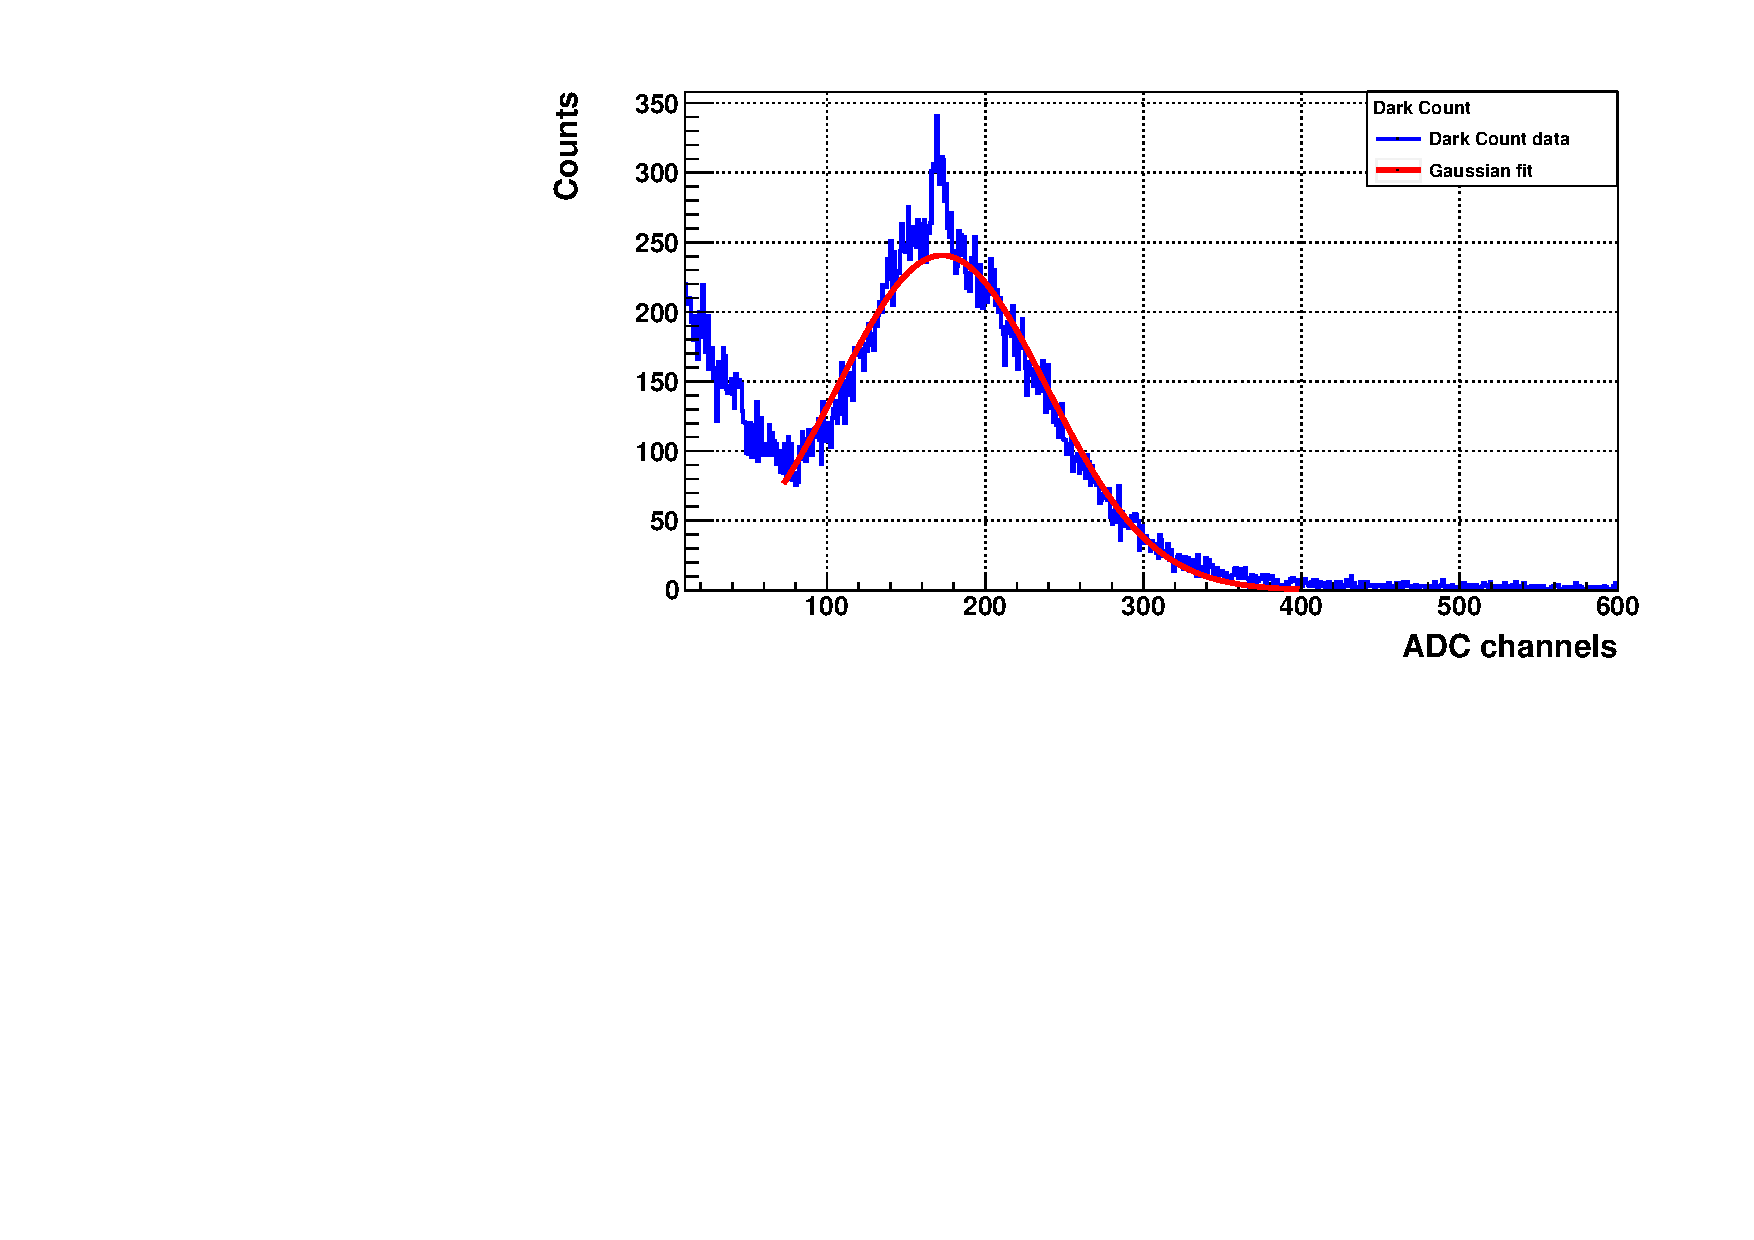
\includegraphics[width=\textwidth]{7ExperimentalResultsDetectors/71ExperimentalResultsLaboratory/714TRITIUMIFIC2/SinglePhotonDistribution.pdf}  
    \caption{\label{subfig:SinglePhotonDistributionIFIC2}}
    \end{subfigure}
    \hfill
    \begin{subfigure}[b]{0.73\textwidth}
    \centering
    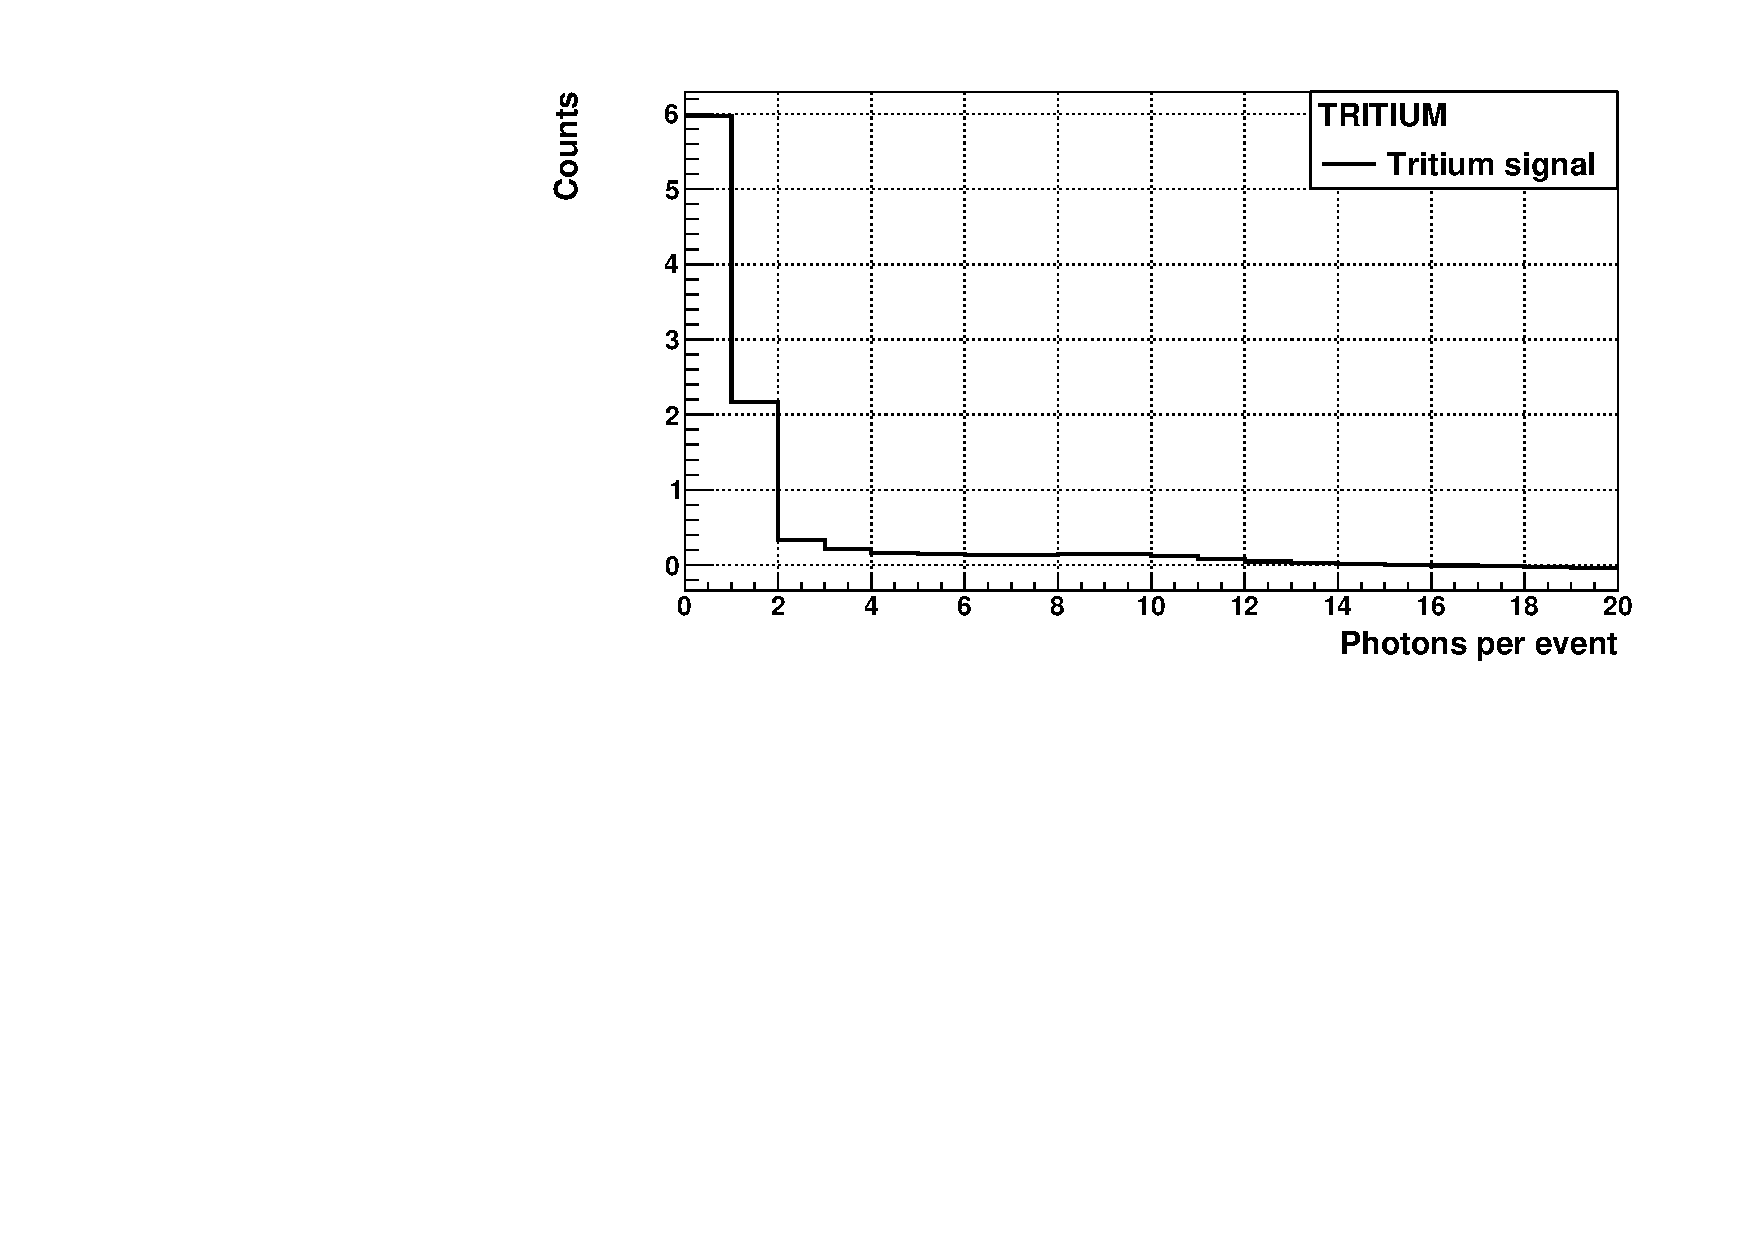
\includegraphics[width=\textwidth]{7ExperimentalResultsDetectors/71ExperimentalResultsLaboratory/714TRITIUMIFIC2/PhotonsPerTritiumEvent.pdf}  
    \caption{\label{subfig:TritiumSignalTRITIUMIFIC2}}
    \end{subfigure}
 \caption{a) Single photon distribution measured with TRITIUM-IFIC 2 prototype. b) Tritium energy spectrum measured with TRITIUM-IFIC 2 prototype in photons detected per event.}
 \label{fig:PhotonsPerTritiumEventIFIC2}
\end{figure}

%\begin{figure}[h]
%\centering
%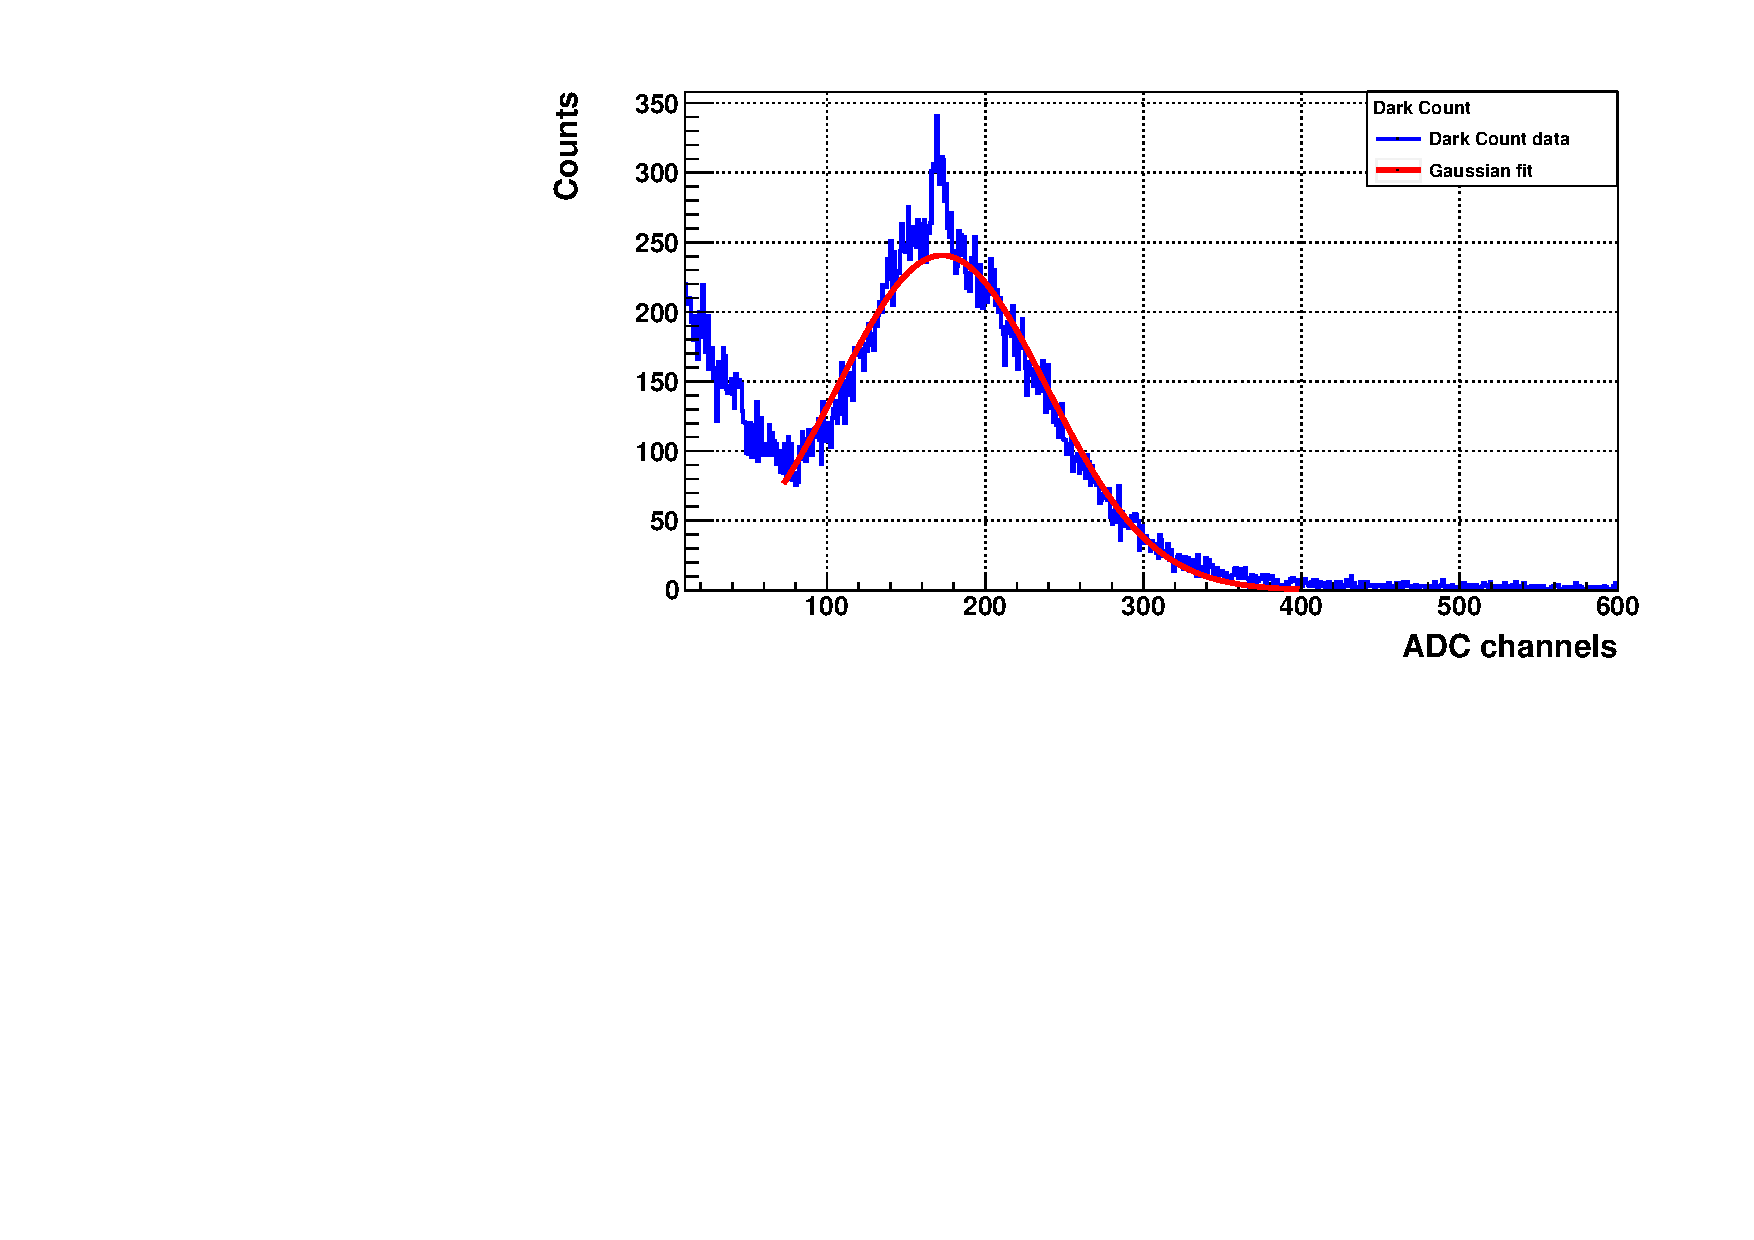
\includegraphics[scale=0.6]{7ExperimentalResultsDetectors/71ExperimentalResultsLaboratory/714TRITIUMIFIC2/SinglePhotonDistribution.pdf}
%\caption{Single photon energy distribution measured with the PMT used in TRITIUM-IFIC 2 prototype.\label{fig:SinglePhotonDistributionIFIC2}}
%\end{figure}

%\begin{figure}[h]
%\centering
%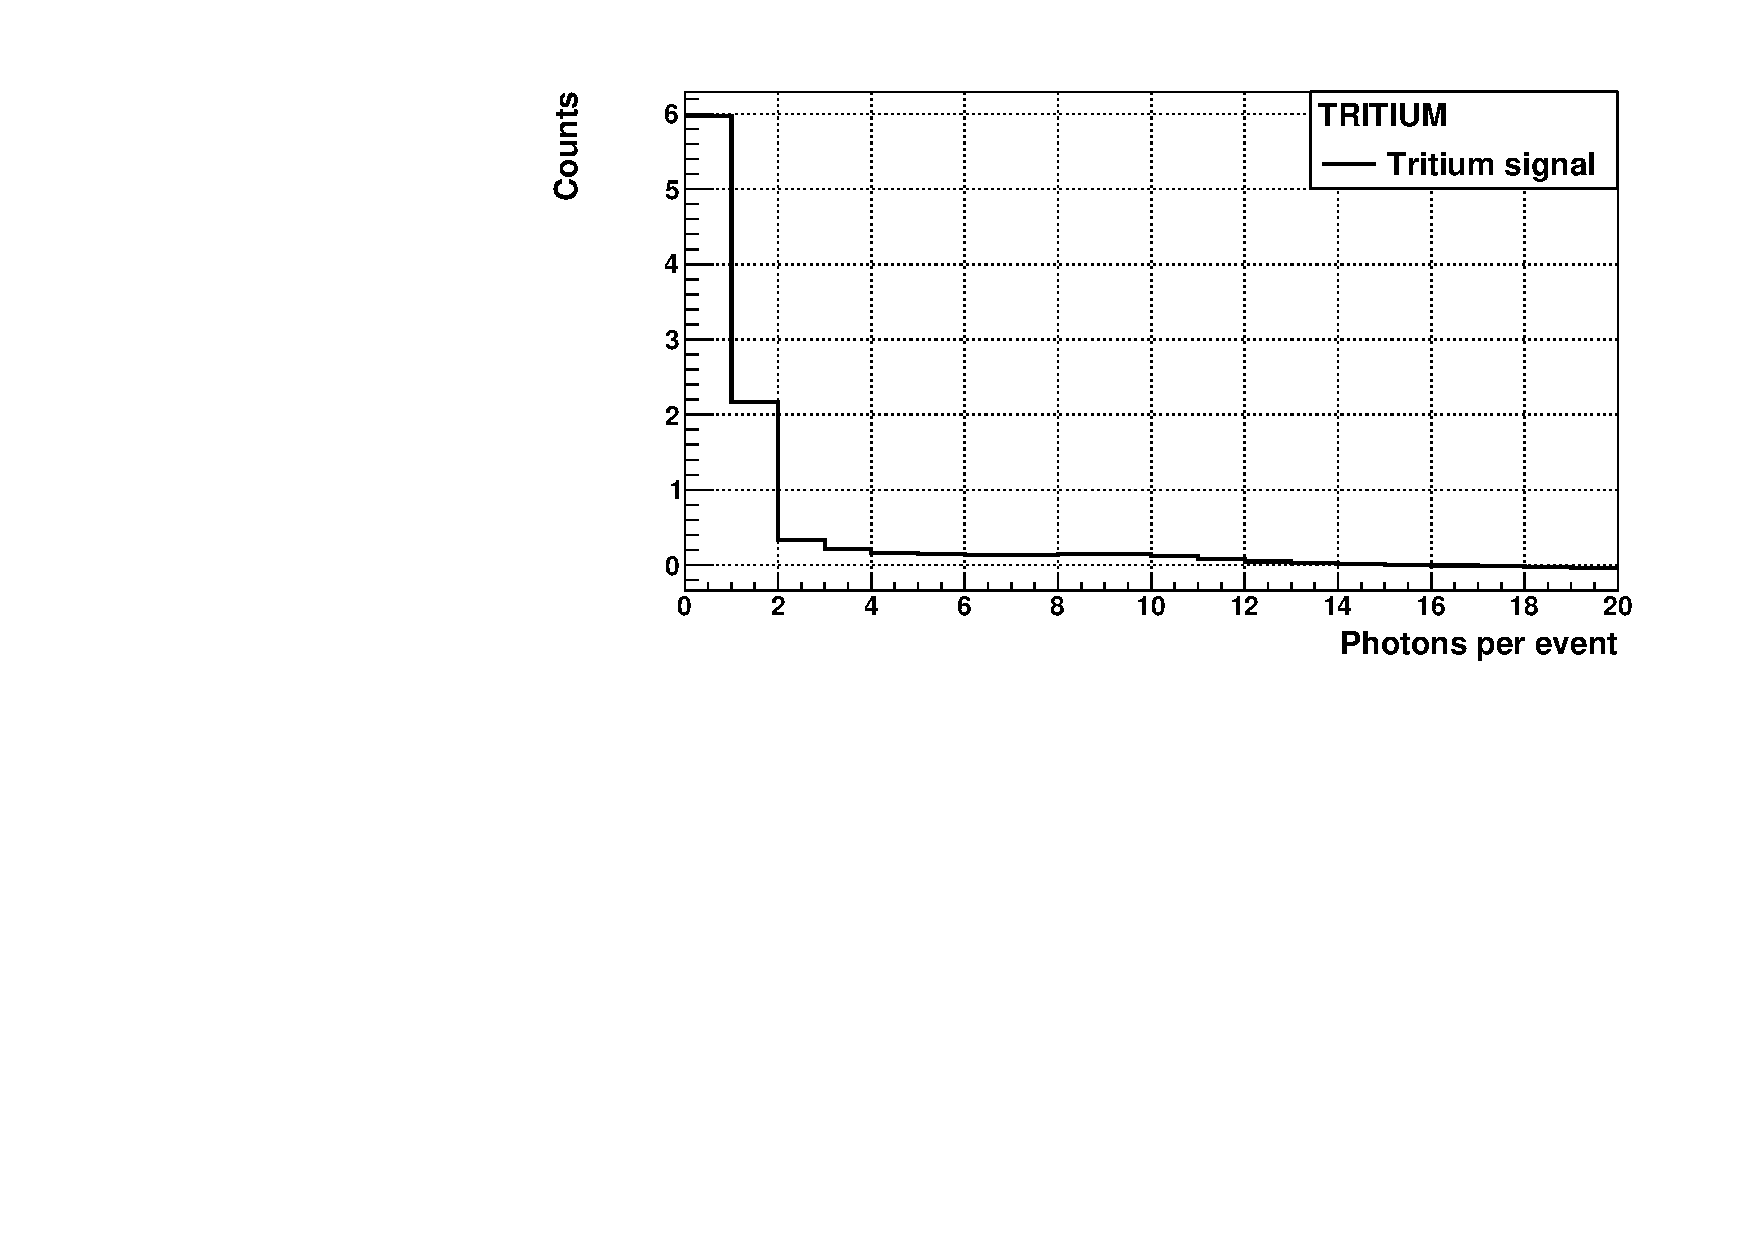
\includegraphics[scale=0.6]{7ExperimentalResultsDetectors/71ExperimentalResultsLaboratory/714TRITIUMIFIC2/PhotonsPerTritiumEvent.pdf}
%\caption{Tritium signal measured with the TRITIUM-IFIC 2 prototype and expressed in number of photones per tritium event detected.\label{fig:TritiumSignalTRITIUMIFIC2}}
%\end{figure}


%As can be seen, a maximum of $15$ photons are generated per tritium event, which corresponds to the best situation. To compare the value obtained with the expected one, the different energies and efficiencies involved are taken into account. Considering a maximum energy for the tritium electron detected, $18.6~\keV$, a scintillation yield of $8000~\text{ph}/\MeV$ for the fibers, a maximum collection efficiency for the fibers, $7\%/\meter$, the fiber length, $20~\cm$ (which increases the collection efficiency by a factor of 5), and the PMT efficiency, $29\%$, the maximum number of photons produced for a tritium event detected with TRITIUM-IFIC 2 prototype is $15$. As can be seen, this is perfectly in accordance with the measurement.

A monitoring of both prototypes, signal and background, were carried out during several months. T rates measured are shown in Figure \ref{fig:MonitorizationTRITIUMIFIC2}.

\begin{figure}[h]
\centering
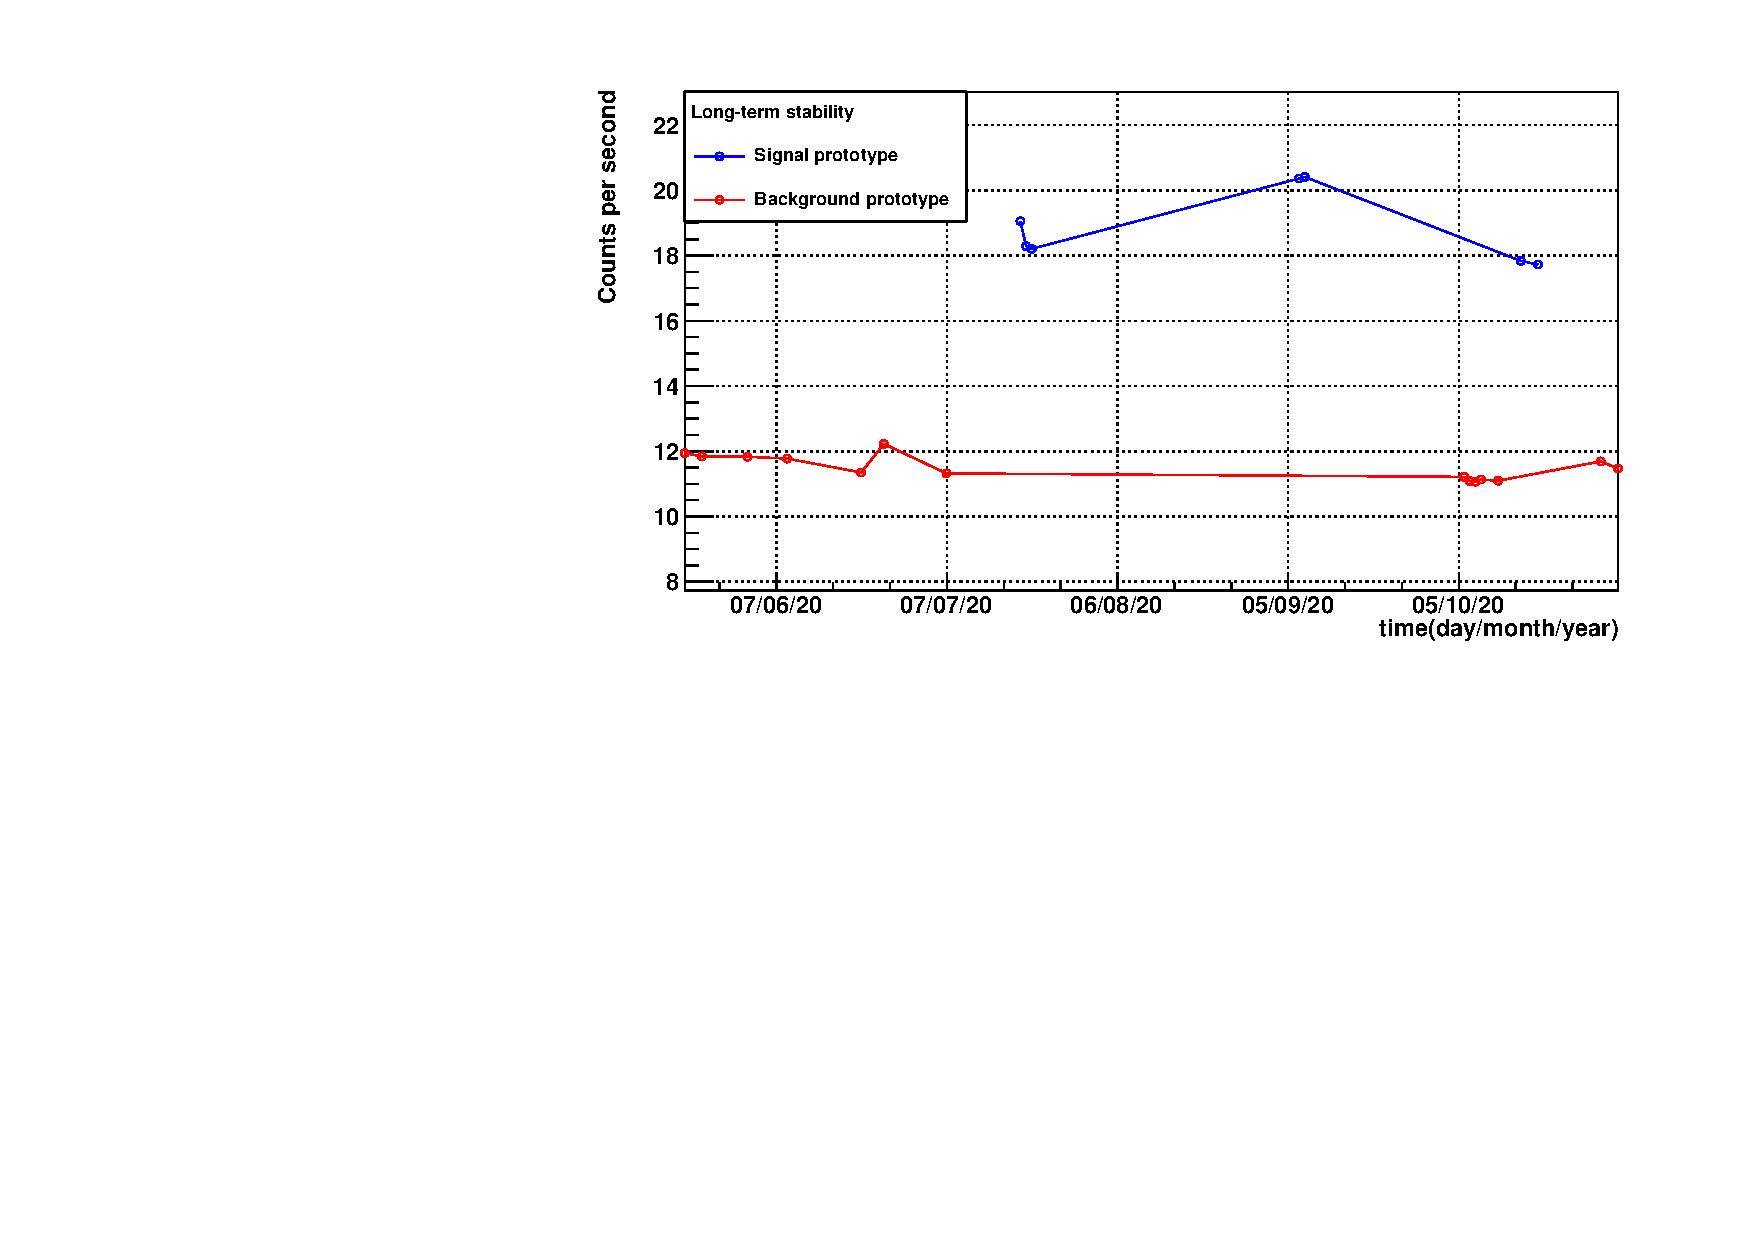
\includegraphics[scale=0.6]{7ExperimentalResultsDetectors/71ExperimentalResultsLaboratory/714TRITIUMIFIC2/Signal_Background_stability_ZOOM.pdf}
\caption{Signal and background rates for a long time measurement.\label{fig:MonitorizationTRITIUMIFIC2}}
\end{figure}
No quenching of the signal was observed, indicating a stability the detector efficiency during 3 months for the signal and 6 months for the background. %Furthermore, it can be verified that the tritium activity used, $10~\kilo\becquerel/\liter$, is not the LDL of the TRITIUM-IFIC 2 prototype since both measurements, signal and background, are clearly separated along the time.

%ESTUDIAR EL LDL DEL DETECTOR CON LAS MEDIDAS TOMADAS!!!

%INCLUIR QUE NO SE HA CONSEGUIDO MEDIR 1kBq/L!!!


%Rellenar con uan actividad grande y volver a medir. 

%Vaciar el prototipo y rellenar con actividades más pequeñas. 1000 y 100 Bq/L.

%Comparar fondos en el laboratorio, caceres, almaraz, etc.

%Medir en el prototipo con SIPM.

%Menos fondo que con el prototipo de AVEIRO en laboratorio Aveiro pero más que en laboratorio extremadura!!!!!!!!!!!!!!!!!!!!